% Please make sure you insert your
% data according to the instructions in PoSauthmanual.pdf
\documentclass{PoS}

\title{Search for High-Energy Neutrinos from Populations of Optical Transients}

\ShortTitle{Neutrinos from Optical Transients}

\author{\speaker{Robert Stein} for the IceCube Collaboration\\
        DESY Zeuthen, Platanenallee 6, 15738 Zeuthen, Germany\\
        E-mail: \email{robert.stein@desy.de}}

%\author{Another Author\\
%        Affiliation\\
%        E-mail: \email{...}}

\abstract{Since the detection of high-energy cosmic neutrinos at the IceCube Neutrino Observatory in 2013, there has been an on-going search to find suitable transient or variable source candidates. Despite recent evidence identifying a flaring blazar as a possible neutrino source, the vast majority of the diffuse neutrino flux measured by IceCube remains unexplained. The latest IceCube results testing time-dependent correlation between neutrinos and Tidal Disruption Events (TDEs) are presented, limiting the contribution of jetted and non-jetted TDEs of the diffuse astrophysical neutrino flux to be less than 1.3\% and 26\% respectively. In addition, a dedicated search for neutrinos from the extraordinary transient AT2018cow are presented, and upper limits on the integrated neutrino emission are derived. Expected improvements from new and upcoming time domain optical surveys (such as ZTF and LSST) are also introduced.}

\FullConference{The New Era of Multi-Messenger Astrophysics - Asterics2019\\
		25 - 29 March, 2019\\
		Groningen, The Netherlands}


\begin{document}
	
\section{Introduction}

The IceCube Neutrino Observatory is a cubic-kilometer array buried 1.5 km beneath glacier ice at the geographic south pole \cite{Aartsen:2016nxy}. When neutrinos undergo charged-current  or neutral-current interactions in the ice, daughter leptons emit Cherenkov light that can be detected by IceCube's 5160 Detector Optical Modules (DOMs). In 2013, IceCube discovered a diffuse flux of high-energy astrophysical neutrinos \cite{Aartsen:2013jdh}, and there has since been an ongoing search to find potential source candidates. Auto-correlation analyses searching for steady neutrino sources, neutrino flares or coincident neutrino multiplets have so far failed to find any significant clustering within the neutrino flux (e.g  \cite{Aartsen:2016oji}). The consistency of this flux with an isotropic distribution suggests that it has a predominantly extragalactic origin. 

 Neutrino astronomy is generally limited by the overwhelming background flux of atmospheric neutrinos, but this can be overcome with two complementary approaches. In the neutrino-driven approach, neutrino data is used to search for possible counterparts. Such an approach forms the basis of the IceCube Realtime Program, in which likely astrophysical neutrinos are identified in real-time and immediately distributed as "alerts" to astronomers \cite{Aartsen:2016lmt}. One succesful example was the follow-up of IC170922A, a high-energy neutrino that was found in coincidence with a flaring blazar, for which a chance association was disfavoured at the level of 3$\sigma$ \cite{IceCube:2018dnn}. However, because only a handful of neutrinos are identified with these filters each year, it can be hard to make statistically-signficant statements about source populations using this approach. These searches are further hampered by the abundance of undetected counterparts that would be expected for most neutrino source populations.

In the alternative source-driven approach, pre-defined catalogues are tested for excesses in neutrinos, with the required spatial coincidence significantly reducing the background for searches. Additionally requiring temporal coincidence, either with the lifetime of a transient, or during  pre-defined "interesting periods" for variable objects, can further reduce background. Multiple sources can be combined in a stacking analysis, which are designed to detect the sum of many weak individual sources. In all cases, these methods rely on multi-messenger and multi-wavelength observations to identify sources to be analysed. Despite IC170922A, previous IceCube analysis has limited the cumulative distribution of Fermi blazars to the astrophysical neutrino flux to be less than 30\% \cite{Aartsen:2016lir}. The origin of the vast majority of the diffuse neutrino flux thus remains, as yet, undiscovered. Dedicated searches targeting likely sources, including Gamma-Ray Bursts (GRBs), Core-Collapse Supernovae (CCSNe), starburst galaxies and galactic emission, have so far failed to reveal any significant excess above background expectations \cite{Stasik2018Search}. This motivates the continued analysis of new, untested source classes in an attempt to identify the origin of astrophysical neutrinos.

\section{Tidal Disruption Events}

Within this context, a new analysis was undertaken to search for neutrinos from Tidal Disruption Events (TDEs). A TDE occurs when a star approaches a supermassive black hole (SMBH) on a parabolic orbit \cite{Komossa:2015qya}. As gravitational acceleration follows a $\frac{1}{r^{2}}$ dependence, the near side of the star will be accelerated more strongly than the far side. The star thus experiences a net tidal force. As the star moves closer to the SMBH, the tidal force increases, until it exceeds the self-gravity that holds the star together. At this point, the star is said to be tidally-disrupted, and roughly half of the stellar debris is accreted. In some cases, a relativistic jet can be formed during the accretion process, analagously to a blazar jet. There has been recent theoretical interest in TDEs as potential Ulta-High Energy Cosmic Ray (UHECR) sources, as well as candidate neutrino sources (e.g \cite{Biehl:2017hnb}).

TDEs are a fundamentally rare phemomenon, with rates several orders of magnitude below CCSN rates \cite{vanVelzen:2017qum}. However, historically poor detection efficiences have further exacerbated this, leaving only a handful of reliably-identified TDEs. To date, there have been only 3 on-axis jetted TDEs, and a few dozen candidate non-jetted TDEs \cite{Komossa:2015qya, Auchettl:2016qfa}. Of these, the majority do not have an unambiguous TDE classification. TDEs themselves are, by their nature, nuclear transients. They can often be confused with flares of Active Galactic Nuclei (AGN), as well as nuclear CCSNe. Due to the greater abundance of these background populations, it can be hard to remove all contamination. Ultimately muliple eras of spectroscopy and photometry are required for a compelling classification. At the time of catalogue compilation in October 2017 \cite{Auchettl:2016qfa}, out of approximately 60 candidate TDEs in the literature overlapping IceCube data-taking, only 13 were judged to be unambiguously classified. 

\section{Results}
\subsection{Stacking Search}

The stacking method employed for the analysis did not make assumptions on the relative strength of each tested source, and was thus robust against both catalogue contamination and deviations from a standard-candle neutrino emission scheme \cite{Stasik2018Search}. However, in order to meaningfully interpret the results, and extrapolate to constrain emission from the population as a whole, a pure sample is required. Consequently, the non-jetted sample was separated based on robustness of classification, with the "Golden TDEs" being assumed representative of non-jetted TDEs as a whole. The results are shown in Figure \ref{fig:DiffuseFlux}. Assuming central rate estimates from \cite{vanVelzen:2017qum} and \cite{Sun:2015bda}, we find that non-jetted and jetted TDEs contribute less than 26\% and 1.3\% respectively to the astrophysical neutrino flux. As the contribution from a population is directly proportional to the local population rate, the shaded bands indicate the uncertainty in our limits arising from rate estimates. For TDEs, these rates are the dominant source of uncertainty in neutrino flux. It will require systematic evaluation of observed TDE rates to enable more precise limits on neutrino emission. Any refined rate estimate can be immediatly used to diretly recalculate  limits, without requiring any additional IceCube analysis.

\begin{figure}[!ht]
	\centering 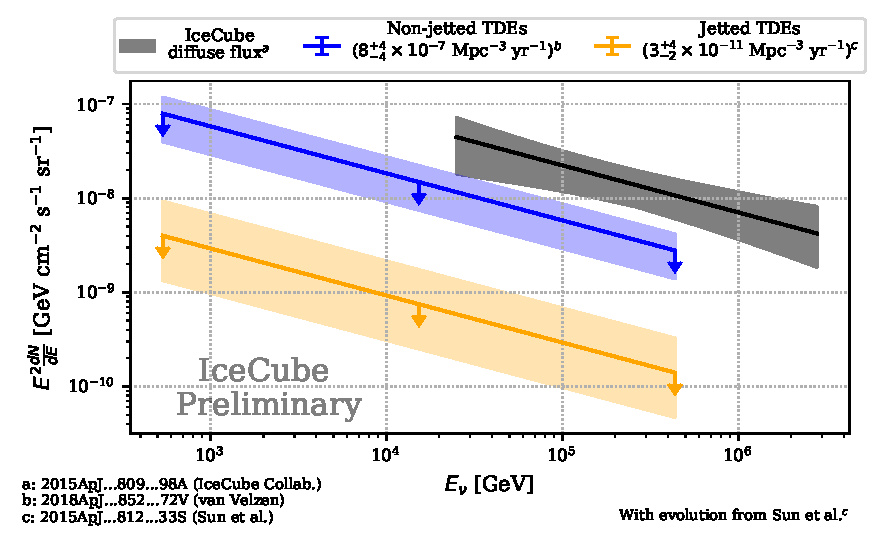
\includegraphics[width=\textwidth]{figures/diffuse_flux_global_fit.pdf}
	\caption{Limits on the contribution of jetted and non-jetted TDEs to the diffuse neutrino flux, assuming standard-candle neutrino emission. The shaded bands represent uncertainty in local rate estimates.}
	\label{fig:DiffuseFlux}
\end{figure}

\subsection{AT2018cow}

The discovery of extraordinary transient AT2018cow was a further demonstration of the central importance of multi-messenger observations.  This fast, bright, blue transient prompted a comprehensive multi-messenger follow-up campaign, and was variously interpreted as a TDE, an extreme SN or a Magnetar \cite{Perley:2018oky}. The observations were consistent with a nearby example of a recently-identified population of Fast Blue Optical Transients (FBOTs). A new analysis of AT2018cow, extending from 30 days before peak to 100 days afterwards, did not reveal any significant neutrino emission. The corresponding constraints are illustrated in Figure \ref{fig:At2018cow}. As before, uncertainty in both classification and rate estimates hinder attempts to constrain neutrino emission from FBOTs.

\begin{figure}[!ht]
	\centering 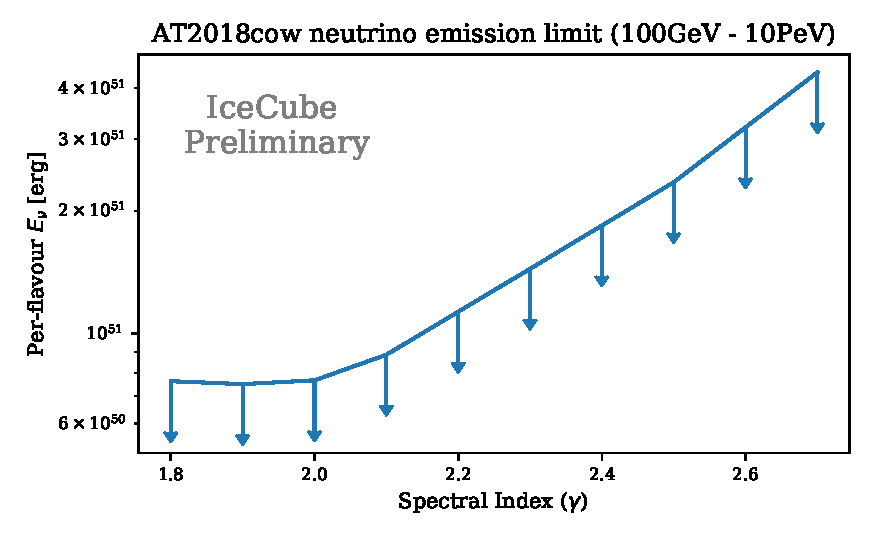
\includegraphics[width=\textwidth]{figures/AT2018cow_limit_plot.pdf}
	\caption{Limits on integrated neutrino emission from AT2018cow as a function of spectral index, assuming a 130 day window from MJD 58256.9 to MJD 58386.9}
	\label{fig:At2018cow}
\end{figure}

\section{Outlook}

The emergence of new telescopes such as ZTF \cite{2019PASP..131a8002B}, as well as upgoing surveys such as LSST, should aid future analysis. By discovering larger numbers of transients, the sensitivity of searches will grow. Larger samples should also improve rate estimation. Higher cadence observations can greatly reduce background by constraining search windows with greater precision. Consequently, source-driven analysis will continue to grow more powerful.

\bibliographystyle{JHEP}
\bibliography{my-bib-database}

\end{document}
